\documentclass[conference]{IEEEtran}
\usepackage[T1]{fontenc}
\usepackage{amsmath,amssymb}
\usepackage{booktabs}
\usepackage{graphicx}
\usepackage{tikz}
\usetikzlibrary{decorations.pathreplacing}
\usepackage[hidelinks]{hyperref}
\newcommand{\code}[1]{\texttt{\small #1}}

\title{Distance Is Not Identity: Cross-Instruction Value Forwarding in
EgDiff's Untagged Speculative Value Queue}
\author{\IEEEauthorblockN{Anonymous Submission}\\
\IEEEauthorblockA{Anonymous Workshop on Hardware Security}}

\begin{document}
\maketitle

\begin{abstract}
Global load-value predictors guess a load's result from an earlier,
different load plus a learned offset. EgDiff (ISCA 2026) makes this
practical with a compact table, a speculative global value queue, and
commit-stage distance polling. Its performance is evaluated; its
security is not. We ask a narrow question: because every dispatched
load receives a queue entry and the base operand is selected solely by
dynamic distance, with no base tag or producer identity, can one
instruction's value be forwarded into another instruction's register
across a software boundary?

We answer yes in a gem5 model, under a same-process non-disclosure
convention. The attacker needs no mispredicted branch in the victim, no
victim-side value-to-address gadget, and no predictor-table collision.
We recover a crafted 64-bit value and the last 8-byte word of a
Monocypher \code{crypto\_verify32} key through the speculative queue,
with zero non-speculative-queue bases, and same-binary controls that
recover nothing. The required code shape occurs in end-loading
comparisons and lookups ($d=1$--$7$) and is absent from the block
primitives we measured ($d\ge 85$). This is a design-level
vulnerability analysis in a simulator, not a hardware or real-world
exploit.
\end{abstract}

\begin{IEEEkeywords}
value prediction, microarchitectural security, speculative execution,
gem5, cache side channel
\end{IEEEkeywords}

\section{Introduction}

Value prediction (VP) breaks true data dependencies by guessing an
instruction's result before it executes. A local predictor uses the
history of one static instruction; a global predictor uses values
produced by other dynamic instructions. Local predictors dominate both
the performance and security literature. EgDiff~\cite{egdiff} revisits
global prediction with a compact table, a speculative value queue, a
3-bit confidence counter, commit-stage training, and deferred
prediction. It reports a 4.37\% average IPC speedup with more than 99\%
accuracy; it does not evaluate security.

The design contains a structural choice that deserves scrutiny.
Section III-B of the paper states:

\begin{quote}\small
``Regardless of whether the prediction is valid or not, a new entry is
allocated in the speculative queue for all candidates.''
\end{quote}

and

\begin{quote}\small
``The speculative queue is then accessed using the distance info to
retrieve the base value. The predicted value is computed as the sum of
the base value and the stride value.''
\end{quote}

The queue entry in Table~I has a value, a distance, a diff, and flags
for valid prediction, misprediction, availability, and wake. It has no
base PC, no base tag, and no producer identity. A load's queue position
is its position in the dynamic load stream.

The security question follows. If the queue is shared and
position-indexed, and the base is selected only by distance, then a load
can consume the value of \emph{any} load that happens to sit $d$
positions earlier. It need not be the same static instruction, and it
need not write a register the consumer reads. That is a cross-instruction
forwarding primitive: the identity of the producer is replaced by a
number.

\paragraph{Contributions.}
\begin{enumerate}
\item We identify the untagged, distance-selected base as the
security-relevant property of EgDiff. Prior value-predictor attacks rely
on a table collision between attacker and victim, or on a victim-side
value-to-address gadget. The global queue removes both.
\item We implement EgDiff in gem5 and demonstrate the primitive on a
crafted victim and on Monocypher's real \code{crypto\_verify32}, through
the speculative queue only.
\item We separate the mechanism from the observation. The forwarding is
register-level; the observation is a speculative cache fill that
survives the squash in gem5. We test it with a branch-squash control, an
address-delay sweep, and a latency matrix.
\item We measure the precondition on real binaries: end-loading
comparisons and lookups satisfy $d\le 32$; block ciphers and keyed
hashes do not.
\item We state the boundary: a design-level vulnerability analysis under
a source-level non-disclosure convention, not a hardware exploit, a
privilege boundary, or a defence evaluation.
\end{enumerate}

\paragraph{What this paper does not claim.}
The attacker and victim share an address space. The victim's value is
not architecturally \emph{nameable} by the attacker's code, but a native
same-process attacker could read it directly. We do not demonstrate a
privilege or cross-process boundary, a full 32-byte key, a hardware
result, or a defence. We do not claim that the 117 conformance
assertions prove fidelity; most are trace-presence checks.

\section{Background}

\subsection{Structures}
The predictor table has 4,096 entries, each with a 14-bit tag, 2-bit
usefulness, 3-bit forward probabilistic counter (FPC), 64-bit diff, and
5-bit distance. The global value queue (GVQ) has 64 entries: 32
speculative entries that mirror the load queue (LQ), and 32
non-speculative entries that hold committed values. The speculative
segment is allocated and squashed in lockstep with the LQ. On a squash,
entries younger than the squash point are invalidated. At commit, the
value is pushed into the non-speculative segment and used to train the
table.

\subsection{Prediction and distance}
At dispatch, the PC indexes the table. If the tag matches and the FPC is
7, the stored distance and diff are used. The base comes from the
speculative queue at index $\mathit{curIdx}-d$, where $\mathit{curIdx}$
is the new load's slot index before it is pushed. The predicted value is
$\mathit{base}+\mathit{diff}$. If the base is in flight with no value,
EgDiff binds a one-to-one wake field and publishes when the base
completes. At commit, Algorithm~1 computes the actual stride
$v_{\mathrm{actual}}-\mathrm{NVQ}[d]$, compares it with the predicted
diff, and either increments confidence or resets it, decrements the
distance, and recomputes the stride.

\subsection{Deferred prediction and latency}
The paper specifies a normal prediction latency of 3 cycles and a
deferred prediction latency of 2 additional cycles. Our model uses a
pending-publish stage: the destination register is not marked ready
until the publish tick, and commit and squash cancel outstanding
publishes. The attack gates run at the default zero latency; a separate
matrix turns the paper's $+3/+2$ on.

\begin{figure*}[t]
\centering
\resizebox{\textwidth}{!}{%
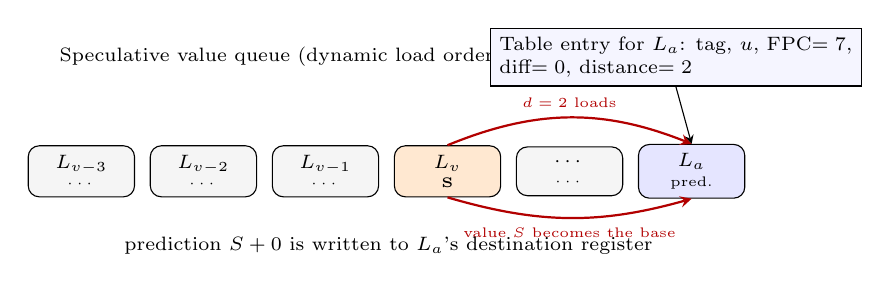
\begin{tikzpicture}[font=\scriptsize,>=stealth]
\node[draw,align=center,rounded corners,minimum width=1.35cm,minimum height=0.62cm,fill=gray!8] (q0) at (0,0) {$L_{v-3}$\\[-1pt]\tiny $\cdots$};
\node[draw,align=center,rounded corners,minimum width=1.35cm,minimum height=0.62cm,fill=gray!8] (q1) at (1.55,0) {$L_{v-2}$\\[-1pt]\tiny $\cdots$};
\node[draw,align=center,rounded corners,minimum width=1.35cm,minimum height=0.62cm,fill=gray!8] (q2) at (3.10,0) {$L_{v-1}$\\[-1pt]\tiny $\cdots$};
\node[draw,align=center,rounded corners,minimum width=1.35cm,minimum height=0.62cm,fill=orange!18] (q3) at (4.65,0) {$L_v$\\[-1pt]\tiny $\mathbf{S}$};
\node[draw,align=center,rounded corners,minimum width=1.35cm,minimum height=0.62cm,fill=gray!8] (q4) at (6.20,0) {$\cdots$\\[-1pt]\tiny $\cdots$};
\node[draw,align=center,rounded corners,minimum width=1.35cm,minimum height=0.62cm,fill=blue!10] (q5) at (7.75,0) {$L_a$\\[-1pt]\tiny pred.};
\node[anchor=west,font=\scriptsize] at (-0.4,1.45) {Speculative value queue (dynamic load order)};
\draw[->,thick,red!70!black] (q3.north) to[bend left=22] node[above,font=\tiny]{$d=2$ loads} (q5.north);
\node[draw,align=left,font=\scriptsize,fill=blue!4] (te) at (7.55,1.45) {Table entry for $L_a$: tag, $u$, FPC$=7$,\\ diff$=0$, distance$=2$};
\draw[->] (te.south) -- (q5.north);
\draw[->,thick,red!70!black] (q3.south) to[bend right=16] node[below,font=\tiny]{value $S$ becomes the base} (q5.south);
\node[font=\scriptsize,align=center] at (3.9,-0.95) {prediction $S+0$ is written to $L_a$'s destination register};
\end{tikzpicture}}
\caption{The attack's carrier. Every candidate load gets a queue slot;
the attacker's table entry selects a base by distance alone. The
victim's slot has no identity check, so its value becomes the attacker's
base.}
\label{fig:queue}
\end{figure*}

\section{Threat Model}

We assume a single core, a single thread, and a single address space.
The victim is an in-process component: a library routine, a sandbox/JIT
host helper, or a cryptographic check. The attacker controls its own
code and the call site, including the loads it executes after the call
returns. The victim's sensitive value is loaded by the victim, used in
registers, and not returned to the caller. The attacker's measurement
path has no architectural reference to the value.

The non-disclosure convention is instantiated in the artifact. The
target value is a \code{static} object in a separate translation unit.
The attacker translation unit has no undefined reference to a
\code{secret\_*} or \code{v32\_key} symbol, and the attacker calls only
the public helper. This is \emph{not} an MMU or sandbox boundary, and we
do not present it as one. The symbol check proves non-naming, not
non-reading. A native same-process attacker could compute the address
from the target's code, scan \code{.rodata}, or use
\code{/proc/self/mem}.

The observable is a speculative cache fill. The dependent probe issues
with the forwarded value before the mispredicting load's data access and
verification. The probe's line survives the squash in gem5; the attacker
later times 256 lines and reads the encoded byte.

\section{Attack Design}

\paragraph{Training.}
The attacker trains its own table entry to a chosen distance $d$ and
offset zero. The training body is structured so that no other distance
is a fixed point: a carrier load whose value equals the attacker's load
sits exactly $d$ loads earlier, and all other loads vary. Algorithm~1
therefore walks to $d$ and latches diff $=0$.

\paragraph{Forwarding.}
The attacker calls the victim once and executes its load immediately
after the return. If the victim's secret load is $d$ positions earlier,
the predictor uses that slot as the base and forwards
$\mathit{secret}+0$ into the attacker's destination register. The victim
contains no branch, comparison, or address that depends on the secret.

\paragraph{Observation.}
The attacker's load has a delayed address (12 register-only divisions),
so its data access and verification are late. A dependent probe load uses
the forwarded value as an index into a 256-line array and fills one cache
line. When the marker's actual value (a sentinel) arrives, the model
reports a value misprediction and squashes the younger window. The fill
is not rolled back. The attacker scans the array with \code{rdcycle} and
accepts a byte only when exactly one line is clearly hot and the winner
has at least two votes and twice the runner-up's count; otherwise it
reports the byte as unknown.

\begin{figure}[t]
\centering
\resizebox{\columnwidth}{!}{%
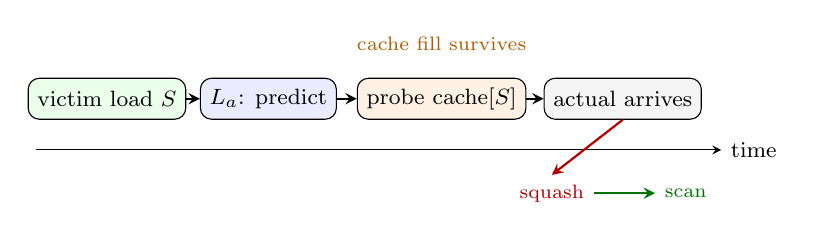
\begin{tikzpicture}[font=\footnotesize,>=stealth]
\draw[->] (0,0) -- (8.7,0) node[right]{time};
\node[draw,rounded corners,fill=green!8,minimum width=1.55cm,minimum height=0.52cm] (v) at (0.9,0.65) {victim load $S$};
\node[draw,rounded corners,fill=blue!8,minimum width=1.65cm,minimum height=0.52cm] (d) at (2.95,0.65) {$L_a$: predict};
\node[draw,rounded corners,fill=orange!10,minimum width=2.0cm,minimum height=0.52cm] (p) at (5.15,0.65) {probe cache[$S$]};
\node[draw,rounded corners,fill=gray!8,minimum width=1.8cm,minimum height=0.52cm] (a) at (7.45,0.65) {actual arrives};
\draw[->,thick] (v) -- (d);
\draw[->,thick] (d) -- (p);
\draw[->,thick] (p) -- (a);
\node[font=\scriptsize,text=red!70!black] (s) at (6.55,-0.55) {squash};
\node[font=\scriptsize,text=green!45!black] (r) at (8.25,-0.55) {scan};
\draw[->,thick,red!70!black] (a.south) -- (s.north);
\draw[->,thick,green!45!black] (s.east) -- (r.west);
\node[font=\scriptsize,text=orange!70!black,align=center] at (5.15,1.35) {cache fill survives};
\end{tikzpicture}}
\caption{Transient timeline. The probe's cache access is earlier than the
marker's verification. The register write is squashed; the cache line is
not.}
\label{fig:timeline}
\end{figure}

\section{Methodology}

\paragraph{Model.}
We implement EgDiff in gem5: the 4,096-entry table, 32-entry
speculative queue, Algorithm~1, the FPC, the 1,024-instruction
suppression window, and the deferred wake. The attack runs use the
default gem5 configuration: 2~GHz, 64~KiB 2-way L1D, no L2/L3,
TournamentBP, and 256/256 physical registers. A separate SPEC
sensitivity run uses the paper's core/cache shape: 4~GHz, 32~KiB 4-way
L1, 256~KiB L2, 2~MiB L3, L-TAGE, 168/168 registers, and
192/64/32/32 ROB/IQ/LQ/SQ. The ISA is RISC-V; the paper uses ARMv8-A.

\paragraph{Metrics.}
\begingroup\raggedright
Coverage is the ratio of \code{egdiffCommittedPredicted} to
\code{egdiffCommits}. Accuracy is \code{egdiffCommittedPredicted}
divided by \code{egdiffCommittedPredicted} plus
\code{numPredictionIncorrect}. The numerator is commit-based; the
denominator also counts wrong-path loads that verified incorrectly, so
the two are not a strict partition. Dispatch-time ratios are diagnostic
only.
\par\endgroup

\paragraph{Distance.}
$d$ is the number of dynamic \emph{load} instructions from the producer
to the consumer, 1-based. If $n$ loads execute strictly between the last
sensitive load and the caller's marker, $d=n+1$. Stores and ALU
operations do not advance the queue.

\paragraph{Controls.}
The main controls are same-binary: \code{EGDIFF\_ON=0} and
\code{EGDIFF\_TYPE=flop}. Both run the same ELF, victim, and measurement
loop. The A4 gate also requires \code{egdiffNVQBases=0}, so every
reported base is in the speculative queue.

\section{Results}

\subsection{Crafted forwarding}
The crafted Mode~1 victim loads a 64-bit static value and returns. The
attacker recovers five different 64-bit values with \code{known=ff},
including values composed of the estimator's sentinel bytes. The off and
FLOP controls recover nothing with \code{known=00} (Table~\ref{tab:crafted}).
This is a controlled demonstration of the primitive, not a real target.

\begin{table}[h]
\centering\small
\caption{Crafted Mode~1.}
\label{tab:crafted}
\begin{tabular}{@{}lccc@{}}
\toprule
run & recovered & known & verdict\\
\midrule
EgDiff on & 64-bit secret & ff & MATCH\\
EgDiff off & 0 & 00 & NO-MATCH\\
FLOP & 0 & 00 & NO-MATCH\\
\bottomrule
\end{tabular}
\end{table}

\subsection{Real target: \code{crypto\_verify32}}
A4 targets Monocypher's constant-time \code{crypto\_verify32}. The last
8-byte key word is at $d=7$--$14$ from the caller's marker. The attack
recovers \code{key[24..31] = a1108f2ebd4cdb6a}, 8/8 bytes, 16 votes per
lane, with \code{egdiffNVQBases=0}, \code{base=specgvq}, and a nonzero
\code{base\_pc} naming the key load (Table~\ref{tab:a4}). The strict
gate passes 36/36. The 1- and 4-division variants also recover 8/8; the
2-division run is a measurement false negative.

\begin{table}[h]
\centering\small
\caption{A4 strict SpecGVQ.}
\label{tab:a4}
\begin{tabular}{@{}lcc@{}}
\toprule
quantity & result & control\\
\midrule
recovered word & \code{a1108f2ebd4cdb6a} & off 0/8\\
bytes & 8/8 & FLOP 0/8\\
NVQ bases & 0 & ---\\
\code{base} & \code{specgvq} & ---\\
\bottomrule
\end{tabular}
\end{table}

\subsection{Race, squash, and latency}
The address-delay sweep is a controlled sensitivity. At zero
register-only divisions the attack recovers 3/8 bytes; at one division
it recovers 8/8. The cycle trace puts the probe's cache request
54--185 cycles before verification at one division (average 62), and
115--331 cycles at twelve (average 197). The fill also survives a
branch-misprediction squash: 16 cycles for the touched line versus 116 in
the untouched null. The paper's $+3$ normal / $+2$ deferred latency
matrix (0/0, 3/0, 0/2, 3/2, 5/2) recovers; the trace shows 1,500 ticks
for $+3$ at 2~GHz (Table~\ref{tab:race}).

\begin{table}[h]
\centering\small
\caption{Race and latency controls.}
\label{tab:race}
\begin{tabular}{@{}lcc@{}}
\toprule
configuration & result & margin (cycles)\\
\midrule
0 divisions & 3/8, \code{known=e0} & ---\\
1 division & 8/8 & 54--185 (avg 62)\\
12 divisions & 8/8 & 115--331 (avg 197)\\
$+3/+2$ latency & 8/8 & ---\\
off at $+3/+2$ & NO-MATCH & ---\\
\bottomrule
\end{tabular}
\end{table}

\subsection{Precondition in real code}
Over 6,300 calls in eight functions, end-loading comparisons and
lookups satisfy $d\le 32$: \code{crypto\_verify32} at 7, \code{memcmp}
and \code{strcmp} at 1, synthetic hash lookup and list walk at 2 (1--2).
The measured block primitives do not: \code{crypto\_chacha20} at 519
(min 85), keyed \code{blake2b} at 552 (min 312), and
\code{crypto\_aead\_lock} at 1,339 (min 560). The result is a
precondition measurement, not an attack on those functions.

\subsection{Behavioural sanity on SPEC}
The SPEC run is a first-30M-from-\code{\_start} smoke test, not a
conformance result. With the default config the five available
benchmarks give an unweighted mean of 26.84\% coverage and 98.82\%
accuracy; with the paper-style core/cache config, 26.70\% and 98.77\%.
\code{505.mcf}'s 64.48\% is startup array initialisation; the paper's
Fig.~10(b) shows its steady-state coverage below 10\%. A 200M run of
\code{510.parest} gives 13.27\% / 99.85\%, versus 22.64\% / 99.80\% at
30M, so the window materially changes the number. The paper uses 50M
warm-up + 100M SimPoints; we do not. The test supports ``the model is
not broken,'' not ``the model matches the paper.''

\section{Related Work}

\paragraph{Value-predictor attacks.}
Deng and Szefer show that predictor state can leak by constructing
collisions between attacker and victim predictor indices~\cite{deng}.
Their attack needs the attacker's load to alias the victim's table entry.
EgDiff's attacker does not collide with the victim's entry; it trains its
own entry and selects the victim's value by queue position.

FLOP exploits a local load-value predictor on Apple silicon~\cite{flop}.
The predicted value must ultimately influence a memory access; FLOP's
victim-side gadget supplies that access. In our attack the victim only
loads the secret; the attacker's own probe supplies the address. The
attacker still needs a value-to-address probe, so ``no gadget'' means no
gadget \emph{in the victim}.

\paragraph{Transient execution.}
Spectre~\cite{spectre} uses a mispredicted branch; our attack needs no
branch misprediction in the victim. The observation is a transient cache
fill, so speculative-cache defences such as SafeSpec~\cite{safespec},
Delay-on-Miss, and InvisiSpec are relevant to the observation. They are
not evaluated here; the register-level forwarding would remain even if
the fill were blocked. ISER~\cite{iser} recomputes rather than predicts
values and is a different design point.

\paragraph{Global prediction.}
gDiff~\cite{gdiff} introduced the global value queue. EgDiff replaces its
multiple strides with one stride and a distance field. Our result
concerns the queue's lack of producer identity, not the stride
representation.

\section{Limitations}

\begin{itemize}
\item \textbf{No hardware.} All attack results are gem5. The cache-fill
survival is a model property.
\item \textbf{No real capability boundary.} The attacker is same-process
native code; the non-disclosure convention is not an MMU or sandbox.
\item \textbf{One key word.} A4 recovers \code{key[24..31]}, not the full
32-byte key. The first word is outside the 32-load window.
\item \textbf{Narrow target.} One library and one function; the
\code{memcmp}/\code{strcmp}/lookup/walk rows are precondition
measurements, not attacks.
\item \textbf{Model scope.} The attack runs use 2~GHz, 64~KiB 2-way L1D,
no L2/L3, TournamentBP, and 256/256 registers. The paper uses 4~GHz, a
32~KiB 4-way L1D, L2/L3, and L-TAGE. The SPEC run is a startup smoke
test, not SimPoints.
\item \textbf{No defence.} SafeSpec/DoM are not evaluated; the impact is
conditional on an undefended hierarchy.
\item \textbf{No full timing model.} Predictor latency $+3/+2$ is
modelled; PRF port pressure, write elision, subword handling, and
LQ$>32$ are not.
\end{itemize}

\section{Conclusion}

EgDiff's speculative global value queue is shared, position-indexed, and
untagged, and its base is selected by distance only. That is a
cross-instruction forwarding primitive: an attacker who trains its own
entry to distance $d$ and offset zero receives the value of whatever
load sits $d$ positions earlier, even when that load belongs to another
software component and the victim has no value-to-address gadget. In a
gem5 model, under a same-process non-disclosure convention, the primitive
recovers a crafted 64-bit value and the last 8-byte word of a Monocypher
\code{crypto\_verify32} key through the speculative queue. The design fix
is to tag the queue base with a producer identity and require the
consumer's entry to expect that producer, or to restrict predictions to
bases produced by the load's own PC. We did not measure either fix.

\small
\bibliographystyle{plain}
\begin{thebibliography}{10}
\setlength{\itemsep}{0pt}
\bibitem{egdiff} L. Yang \emph{et al.}, ``Revisiting Global Value
Prediction: A Resurgent Complement to Local Predictors,'' in
\emph{Proc. ISCA}, 2026.
\bibitem{deng} S. Deng and J. Szefer, ``New Predictor-Based Attacks in
Processors,'' in \emph{Proc. MICRO}, 2021.
\bibitem{flop} J. He \emph{et al.}, ``FLOP: Breaking the Apple M3 CPU via
False Load Output Predictions,'' 2025.
\bibitem{spectre} P. Kocher \emph{et al.}, ``Spectre Attacks: Exploiting
Speculative Execution,'' in \emph{Proc. IEEE S\&P}, 2019.
\bibitem{safespec} K. Khasawneh \emph{et al.}, ``SafeSpec: Banishing the
Spectre of a Meltdown with Leakage-Free Speculation,'' in \emph{Proc.
DAC}, 2019.
\bibitem{iser} C. Sakalis \emph{et al.}, ``Efficient Invisible Speculative
Execution through Selective Delay and Value Prediction,'' in
\emph{Proc. ISCA}, 2019.
\bibitem{gdiff} H. Zhou, J. Flanagan, and T. Conte, ``Detecting Global
Stride Value Locality in Program Execution,'' in \emph{Proc. PLDI}, 2003.
\bibitem{monocypher} L. Vaillant, ``Monocypher,'' 2026.
\bibitem{simpoint} T. Sherwood \emph{et al.}, ``Automatically
Characterizing Large Scale Program Behavior,'' in \emph{Proc. ASPLOS},
2002.
\bibitem{spec} SPEC CPU 2017, Standard Performance Evaluation Corporation.
\end{thebibliography}

\end{document}
